\chapter{平方根算法}

\index{平方根算法}

\key{平方根算法}是一种时间复杂度中包含平方根的算法。
平方根可以看作是''穷人的对数''：
复杂度$O(\sqrt n)$比$O(n)$好，
但比$O(\log n)$差。
无论如何，许多平方根算法在实践中是快速且可用的。

例如，考虑这样一个问题：
创建一个支持对数组进行两种操作的数据结构：
修改给定位置的元素
以及计算给定范围内元素的和。
我们之前使用树状数组和线段树
解决了这个问题，
它们都能在$O(\log n)$时间内完成两种操作。
然而，现在我们将使用平方根结构
以另一种方式解决问题，
该结构允许我们在$O(1)$时间内修改元素，
在$O(\sqrt n)$时间内计算求和。

其思想是将数组划分为大小为$\sqrt n$的\emph{块}，
使得每个块包含块内元素的和。
例如，一个包含16个元素的数组
将被划分为每块4个元素，如下所示：

\begin{center}
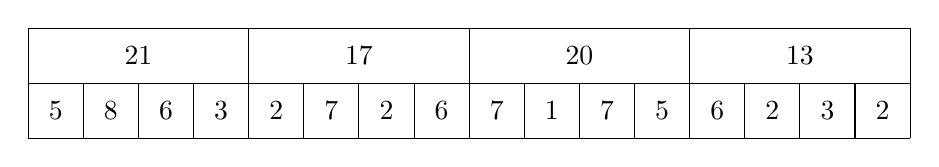
\begin{tikzpicture}[scale=0.7]
\draw (0,0) grid (16,1);

\draw (0,1) rectangle (4,2);
\draw (4,1) rectangle (8,2);
\draw (8,1) rectangle (12,2);
\draw (12,1) rectangle (16,2);

\node at (0.5, 0.5) {5};
\node at (1.5, 0.5) {8};
\node at (2.5, 0.5) {6};
\node at (3.5, 0.5) {3};
\node at (4.5, 0.5) {2};
\node at (5.5, 0.5) {7};
\node at (6.5, 0.5) {2};
\node at (7.5, 0.5) {6};
\node at (8.5, 0.5) {7};
\node at (9.5, 0.5) {1};
\node at (10.5, 0.5) {7};
\node at (11.5, 0.5) {5};
\node at (12.5, 0.5) {6};
\node at (13.5, 0.5) {2};
\node at (14.5, 0.5) {3};
\node at (15.5, 0.5) {2};

\node at (2, 1.5) {21};
\node at (6, 1.5) {17};
\node at (10, 1.5) {20};
\node at (14, 1.5) {13};

\end{tikzpicture}
\end{center}

在这个结构中，
修改数组元素很容易，
因为每次修改后只需要更新
单个块的和，
这可以在$O(1)$时间内完成。
例如，下图显示了一个元素的值
和对应块的和如何变化：

\begin{center}
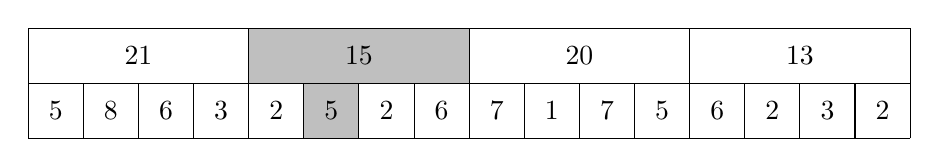
\begin{tikzpicture}[scale=0.7]
\fill[color=lightgray] (5,0) rectangle (6,1);
\draw (0,0) grid (16,1);

\fill[color=lightgray] (4,1) rectangle (8,2);
\draw (0,1) rectangle (4,2);
\draw (4,1) rectangle (8,2);
\draw (8,1) rectangle (12,2);
\draw (12,1) rectangle (16,2);

\node at (0.5, 0.5) {5};
\node at (1.5, 0.5) {8};
\node at (2.5, 0.5) {6};
\node at (3.5, 0.5) {3};
\node at (4.5, 0.5) {2};
\node at (5.5, 0.5) {5};
\node at (6.5, 0.5) {2};
\node at (7.5, 0.5) {6};
\node at (8.5, 0.5) {7};
\node at (9.5, 0.5) {1};
\node at (10.5, 0.5) {7};
\node at (11.5, 0.5) {5};
\node at (12.5, 0.5) {6};
\node at (13.5, 0.5) {2};
\node at (14.5, 0.5) {3};
\node at (15.5, 0.5) {2};

\node at (2, 1.5) {21};
\node at (6, 1.5) {15};
\node at (10, 1.5) {20};
\node at (14, 1.5) {13};

\end{tikzpicture}
\end{center}

然后，要计算一个范围内元素的和，
我们将该范围分为三部分，
使得和由单个元素的值
和它们之间块的和组成：

\begin{center}
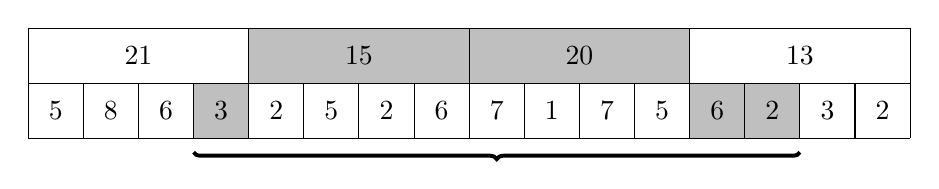
\begin{tikzpicture}[scale=0.7]
\fill[color=lightgray] (3,0) rectangle (4,1);
\fill[color=lightgray] (12,0) rectangle (13,1);
\fill[color=lightgray] (13,0) rectangle (14,1);
\draw (0,0) grid (16,1);

\fill[color=lightgray] (4,1) rectangle (8,2);
\fill[color=lightgray] (8,1) rectangle (12,2);
\draw (0,1) rectangle (4,2);
\draw (4,1) rectangle (8,2);
\draw (8,1) rectangle (12,2);
\draw (12,1) rectangle (16,2);

\node at (0.5, 0.5) {5};
\node at (1.5, 0.5) {8};
\node at (2.5, 0.5) {6};
\node at (3.5, 0.5) {3};
\node at (4.5, 0.5) {2};
\node at (5.5, 0.5) {5};
\node at (6.5, 0.5) {2};
\node at (7.5, 0.5) {6};
\node at (8.5, 0.5) {7};
\node at (9.5, 0.5) {1};
\node at (10.5, 0.5) {7};
\node at (11.5, 0.5) {5};
\node at (12.5, 0.5) {6};
\node at (13.5, 0.5) {2};
\node at (14.5, 0.5) {3};
\node at (15.5, 0.5) {2};

\node at (2, 1.5) {21};
\node at (6, 1.5) {15};
\node at (10, 1.5) {20};
\node at (14, 1.5) {13};

\draw [decoration={brace}, decorate, line width=0.5mm] (14,-0.25) -- (3,-0.25);

\end{tikzpicture}
\end{center}

由于单个元素的数量是$O(\sqrt n)$，
块的数量也是$O(\sqrt n)$，
因此求和查询需要$O(\sqrt n)$时间。
块大小$\sqrt n$的目的是
它\emph{平衡}了两件事：
数组被划分为$\sqrt n$个块，
每个块包含$\sqrt n$个元素。

在实践中，不必使用$\sqrt n$的精确值作为参数，
而是可以使用参数$k$和$n/k$，其中$k$
不同于$\sqrt n$。
最优参数取决于问题和输入。
例如，如果算法经常遍历块
但很少检查块内的单个元素，
那么将数组划分为
$k < \sqrt n$个块，每个块包含$n/k > \sqrt n$
个元素可能是一个好主意。

\section{算法组合}

本节讨论两个平方根算法，
它们基于将两个算法组合为一个算法。
在两种情况下，我们都可以单独使用
其中任一算法
并在$O(n^2)$时间内解决问题。
然而，通过组合算法，运行时间仅为$O(n \sqrt n)$。

\subsubsection{情况处理}

假设给定一个包含$n$个单元格的二维网格。
每个单元格被赋予一个字母，
我们的任务是找到两个具有相同字母的单元格，
使其距离最小，
其中单元格$(x_1,y_1)$和$(x_2,y_2)$之间的距离
为$|x_1-x_2|+|y_1-y_2|$。
例如，考虑以下网格：

\begin{center}
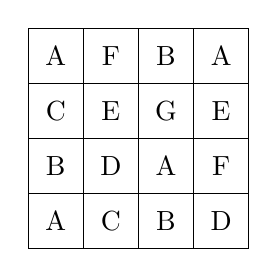
\begin{tikzpicture}[scale=0.7]
\node at (0.5,0.5) {A};
\node at (0.5,1.5) {B};
\node at (0.5,2.5) {C};
\node at (0.5,3.5) {A};
\node at (1.5,0.5) {C};
\node at (1.5,1.5) {D};
\node at (1.5,2.5) {E};
\node at (1.5,3.5) {F};
\node at (2.5,0.5) {B};
\node at (2.5,1.5) {A};
\node at (2.5,2.5) {G};
\node at (2.5,3.5) {B};
\node at (3.5,0.5) {D};
\node at (3.5,1.5) {F};
\node at (3.5,2.5) {E};
\node at (3.5,3.5) {A};
\draw (0,0) grid (4,4);
\end{tikzpicture}
\end{center}
在这种情况下，最小距离为2，是两个'E'字母之间的距离。

我们可以通过分别考虑每个字母来解决问题。
使用这种方法，新问题是计算
具有\emph{固定}字母$c$的两个单元格之间的最小距离。
我们关注两种算法：

\emph{算法1：}遍历所有具有字母$c$的单元格对，
计算这些单元格之间的最小距离。
这需要$O(k^2)$时间，其中$k$是具有字母$c$的单元格数量。

\emph{算法2：}执行广度优先搜索，同时
从每个具有字母$c$的单元格开始。
两个具有字母$c$的单元格之间的最小距离
将在$O(n)$时间内计算出来。

解决问题的一种方法是选择两个算法中的任一个，
并将其用于所有字母。
如果我们使用算法1，运行时间为$O(n^2)$，
因为所有单元格可能包含相同的字母，
在这种情况下$k=n$。
同样如果我们使用算法2，运行时间也是$O(n^2)$，
因为所有单元格可能有不同的字母，
在这种情况下需要$n$次搜索。

然而，我们可以\emph{组合}两种算法，
根据每个字母在网格中出现的次数，
对不同字母使用不同的算法。
假设字母$c$出现$k$次。
如果$k \le \sqrt n$，我们使用算法1；如果$k > \sqrt n$，
我们使用算法2。
事实证明，这样做后，算法的总运行时间仅为$O(n \sqrt n)$。

首先，假设我们对字母$c$使用算法1。
由于$c$在网格中最多出现$\sqrt n$次，
我们将每个具有字母$c$的单元格
与其他单元格比较$O(\sqrt n)$次。
因此，处理所有这些单元格所用的时间为$O(n \sqrt n)$。
然后，假设我们对字母$c$使用算法2。
这样的字母最多有$\sqrt n$个，
因此处理这些字母也需要$O(n \sqrt n)$时间。

\subsubsection{批处理}

我们的下一个问题也涉及
一个包含$n$个单元格的二维网格。
最初，除了一个单元格外，每个单元格都是白色的。
我们执行$n-1$次操作，每次操作首先
计算从给定白色单元格到黑色单元格的最小距离，
然后将该白色单元格涂为黑色。

例如，考虑以下操作：

\begin{center}
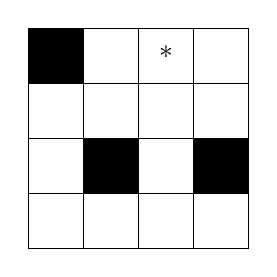
\begin{tikzpicture}[scale=0.7]
\fill[color=black] (1,1) rectangle (2,2);
\fill[color=black] (3,1) rectangle (4,2);
\fill[color=black] (0,3) rectangle (1,4);
\node at (2.5,3.5) {*};
\draw (0,0) grid (4,4);
\end{tikzpicture}
\end{center}

首先，我们计算从标记为*的白色单元格到黑色单元格的最小距离。
最小距离为2，因为我们可以向左移动
两步到达一个黑色单元格。
然后，我们将该白色单元格涂为黑色：

\begin{center}
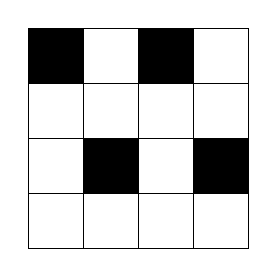
\begin{tikzpicture}[scale=0.7]
\fill[color=black] (1,1) rectangle (2,2);
\fill[color=black] (3,1) rectangle (4,2);
\fill[color=black] (0,3) rectangle (1,4);
\fill[color=black] (2,3) rectangle (3,4);
\draw (0,0) grid (4,4);
\end{tikzpicture}
\end{center}

考虑以下两种算法：

\emph{算法1：}使用广度优先搜索
计算每个白色单元格到最近黑色单元格的距离。
这需要$O(n)$时间，搜索完成后，
我们可以在$O(1)$时间内找到任何白色单元格到黑色单元格的最小距离。

\emph{算法2：}维护一个已被涂为黑色的单元格列表，
在每次操作时遍历该列表，
然后将新单元格添加到列表中。
每次操作需要$O(k)$时间，其中$k$是列表的长度。

我们通过将操作划分为$O(\sqrt n)$个\emph{批}，
每批包含$O(\sqrt n)$次操作，来组合上述算法。
在每批开始时，我们执行算法1。
然后，我们使用算法2处理该批中的操作。
我们在批之间清空算法2的列表。
在每次操作中，
到黑色单元格的最小距离
要么是算法1计算的距离，
要么是算法2计算的距离。

得到的算法在$O(n \sqrt n)$时间内工作。
首先，算法1执行$O(\sqrt n)$次，
每次搜索在$O(n)$时间内完成。
其次，当在一批中使用算法2时，
列表包含$O(\sqrt n)$个单元格
（因为我们在批之间清空列表），
每次操作需要$O(\sqrt n)$时间。

\section{整数划分}

一些平方根算法基于以下观察：
如果将正整数$n$表示为正整数的和，
这样的和最多包含$O(\sqrt n)$个\emph{不同的}数。
原因是，要构造包含最多不同数的和，
我们应该选择\emph{小的}数。
如果我们选择数$1,2,\ldots,k$，
得到的和为
\[\frac{k(k+1)}{2}.\]
因此，不同数的最大数量为$k = O(\sqrt n)$。
接下来我们将讨论两个可以利用这一观察
高效解决的问题。

\subsubsection{背包问题}

假设给定一个整数权重列表，其和为$n$。
我们的任务是找出使用权重子集可以形成的所有和。
例如，如果权重为$\{1,3,3\}$，则可能的和如下：

\begin{itemize}[noitemsep]
\item $0$（空集）
\item $1$
\item $3$
\item $1+3=4$
\item $3+3=6$
\item $1+3+3=7$
\end{itemize}

使用标准背包方法（见第7.4节），
可以如下解决问题：
我们定义函数$\texttt{possible}(x,k)$，如果和$x$可以使用前$k$个权重形成，
则其值为1，否则为0。
由于权重之和为$n$，
最多有$n$个权重，
可以使用动态规划在$O(n^2)$时间内
计算函数的所有值。

然而，我们可以利用最多有$O(\sqrt n)$个\emph{不同的}权重这一事实，
使算法更高效。
因此，我们可以将权重分组处理，
每组由相似的权重组成。
我们可以在$O(n)$时间内处理每组，
从而得到一个$O(n \sqrt n)$时间的算法。

其思想是使用一个数组记录迄今为止已处理过的组
可以形成的权重和。
该数组包含$n$个元素：如果和$k$可以形成，
则元素$k$为1，否则为0。
要处理一组权重，我们从左到右扫描数组，
记录使用该组和之前的组可以形成的新的权重和。

\subsubsection{字符串构造}

给定一个长度为$n$的字符串\texttt{s}
和一个总长度为$m$的字符串集合$D$，
考虑计算\texttt{s}可以由$D$中的字符串拼接
形成的方式数量的问题。
例如，
如果$\texttt{s}=\texttt{ABAB}$且
$D=\{\texttt{A},\texttt{B},\texttt{AB}\}$，
则有4种方式：

\begin{itemize}[noitemsep]
\item $\texttt{A}+\texttt{B}+\texttt{A}+\texttt{B}$
\item $\texttt{AB}+\texttt{A}+\texttt{B}$
\item $\texttt{A}+\texttt{B}+\texttt{AB}$
\item $\texttt{AB}+\texttt{AB}$
\end{itemize}

我们可以使用动态规划解决问题：
令$\texttt{count}(k)$表示使用$D$中的字符串构造前缀
$\texttt{s}[0 \ldots k]$的方式数。
现在$\texttt{count}(n-1)$给出问题的答案，
我们可以使用字典树结构
在$O(n^2)$时间内解决问题。

然而，我们可以利用字符串哈希和$D$中最多有$O(\sqrt m)$种不同字符串长度这一事实，
更高效地解决问题。
首先，我们构造一个集合$H$，包含$D$中所有字符串的哈希值。
然后，在计算$\texttt{count}(k)$的值时，
我们遍历所有使得$D$中存在长度为$p$的字符串的$p$值，
计算$\texttt{s}[k-p+1 \ldots k]$的哈希值
并检查它是否属于$H$。
由于最多有$O(\sqrt m)$种不同的字符串长度，
这会产生一个运行时间为$O(n \sqrt m)$的算法。

\section{Mo's算法}

\index{Mo's算法}

\key{Mo's算法}\footnote{根据\cite{cod15}，该算法
以中国竞赛选手莫涛的名字命名，但
该技术在更早的文献中已经出现\cite{ken06}。}
可用于许多需要在\emph{静态}数组中处理区间查询的问题，
即数组值在查询之间不会改变。
在每个查询中，给定一个范围$[a,b]$，
我们应该根据位置$a$和$b$之间的数组元素
计算一个值。
由于数组是静态的，
查询可以以任何顺序处理，
而Mo's算法以一种特殊的顺序处理查询，
以保证算法高效运行。

Mo's算法维护数组的一个\emph{活动范围}，
在任何时刻都知道与活动范围相关的查询的答案。
算法逐个处理查询，
并通过插入和删除元素
始终移动活动范围的端点。
算法的时间复杂度为
$O(n \sqrt n f(n))$，其中数组包含$n$个元素，
有$n$个查询，每次插入和删除一个元素需要$O(f(n))$时间。

Mo's算法的诀窍在于查询的处理顺序：
数组被划分为$k=O(\sqrt n)$个元素的块，
查询$[a_1,b_1]$
在查询$[a_2,b_2]$之前处理，如果满足以下任一条件：
\begin{itemize}
\item $\lfloor a_1/k \rfloor < \lfloor a_2/k \rfloor$或
\item $\lfloor a_1/k \rfloor = \lfloor a_2/k \rfloor$且$b_1 < b_2$。
\end{itemize}

因此，所有左端点在某个块中的查询
会按右端点排序后依次处理。
使用这种顺序，算法
只需执行$O(n \sqrt n)$次操作，
因为左端点移动$O(n)$次、每次$O(\sqrt n)$步，
右端点移动$O(\sqrt n)$次、每次$O(n)$步。因此，在算法过程中，
两个端点总共移动$O(n \sqrt n)$步。

\subsubsection*{示例}

作为示例，考虑一个问题：
给定一组查询，每个查询对应数组中的一个范围，
我们的任务是计算每个查询对应范围内\emph{不同的}元素数量。

在Mo's算法中，查询始终以相同的方式排序，
但如何维护查询的答案取决于具体问题。
在这个问题中，我们可以维护一个数组
\texttt{count}，其中$\texttt{count}[x]$
表示元素$x$在活动范围内出现的次数。

当我们从一个查询移动到另一个查询时，
活动范围会改变。
例如，如果当前范围为
\begin{center}
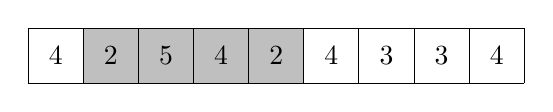
\begin{tikzpicture}[scale=0.7]
\fill[color=lightgray] (1,0) rectangle (5,1);
\draw (0,0) grid (9,1);
\node at (0.5, 0.5) {4};
\node at (1.5, 0.5) {2};
\node at (2.5, 0.5) {5};
\node at (3.5, 0.5) {4};
\node at (4.5, 0.5) {2};
\node at (5.5, 0.5) {4};
\node at (6.5, 0.5) {3};
\node at (7.5, 0.5) {3};
\node at (8.5, 0.5) {4};
\end{tikzpicture}
\end{center}
而下一个范围为
\begin{center}
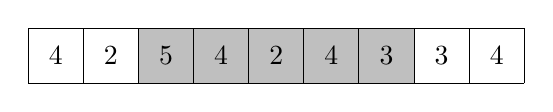
\begin{tikzpicture}[scale=0.7]
\fill[color=lightgray] (2,0) rectangle (7,1);
\draw (0,0) grid (9,1);
\node at (0.5, 0.5) {4};
\node at (1.5, 0.5) {2};
\node at (2.5, 0.5) {5};
\node at (3.5, 0.5) {4};
\node at (4.5, 0.5) {2};
\node at (5.5, 0.5) {4};
\node at (6.5, 0.5) {3};
\node at (7.5, 0.5) {3};
\node at (8.5, 0.5) {4};
\end{tikzpicture}
\end{center}
将有三个步骤：
左端点向右移动一步，
右端点向右移动两步。

每一步之后，都需要更新数组\texttt{count}。
添加一个元素$x$后，
我们将$\texttt{count}[x]$的值增加1，
如果此后$\texttt{count}[x]=1$，
我们还将查询的答案增加1。
类似地，移除一个元素$x$后，
我们将$\texttt{count}[x]$的值减少1，
如果此后$\texttt{count}[x]=0$，
我们还将查询的答案减少1。

在这个问题中，执行每一步所需的时间为$O(1)$，
因此算法的总时间复杂度为$O(n \sqrt n)$。